\documentclass[a4paper,12pt,twoside,titlepage]{article}
\usepackage[pdftitle={Userguide Caesar Development Tools},pdfborder=0,pdfauthor={Jochen Unger, Daniel Zwicker},colorlinks=true,linkcolor=blue,linkbordercolor=255 255 255]{hyperref}
\usepackage{amssymb}
\usepackage{graphicx}
\usepackage[ansinew]{inputenc}
\usepackage{a4}
\usepackage{listings}
\usepackage{color}
\pagestyle{headings}
\usepackage{float}
\restylefloat{figure}
\usepackage{longtable}

\title{\textbf{Userguide Caesar Development Tools}\\\small{Software Technology Group}\\\small{Version 0.9}}
\author{Jochen Unger\and Daniel Zwicker}
%Hier beginnt das Dokument

\newcommand{\code}[1]
{\textbf{"#1"}}

\newcommand{\caesarj}
{\caesar}

\newcommand{\markedtext}[1]
{\fbox{\textbf{#1}}}

\newcommand{\caesar}
{C{\footnotesize AESAR}J}

\newcommand{\jdt}
{Java Development Tool}

\newcommand{\cjdt}
{\caesarj ~Development Tool}

\begin{document}
\lstset{
   frame=l,
   language=Java,
   xleftmargin=10pt, 
   stepnumber=1,
   numbers=left,
   numbersep=5pt,
   numberstyle=\ttfamily\tiny\color[gray]{0.3},
   belowcaptionskip=\bigskipamount,
   escapeinside={*'}{'*},
   tabsize=1,
   emphstyle={\it},
   commentstyle=\rmfamily\it,
   stringstyle=\mdseries\rmfamily,
   showspaces=false,
   keywordstyle=\bfseries,
   columns=flexible,
   basicstyle=\small,
   showstringspaces=false,
   framextopmargin=2pt,
   framexbottommargin=2pt
  }

\maketitle
\tableofcontents

\newpage
\section{Introduction}
This documentation discribes how to use the \caesarj -Eclipse Plugin for the new programming language \caesarj.
\subsection{What is \caesarj ?}
\caesar is a new aspect-oriented programming language that extends JAVA with the following functions:
\begin{itemize}
	\item aspect\footnote{More information about \caesarj ~and aspects read this  \href{http://www.st.informatik.tu-darmstadt.de/database/publications/data/aosd03.pdf?id=70}{Paper}} functionality with runtime deployment of aspects
	\item multible inheritance
	\item produces 100\% pure Java byte code
	\item \dots
\end{itemize}
For more detailed information please visite \href{http://caesarj.org/}{http://caesarj.org/}.

\subsection{Why is a plugin needed?}
\caesarj  extends the Java source code. A pure Java-Editor (e.g. the \jdt -Eclipse Plugin) would not be able to handel this source code. Also the integrated Java compiler would not work. So a IDE is needed, that extends the \jdt. Some features of the \caesarj -Plugin are:
\begin{itemize}
	\item integrated caesarj builder
	\item codehighlighting for \caesarj ~expressions
	\item visualisation of aspects
	\item visualisation of multible inheritance
	\item \dots
\end{itemize}
For detailed describtion please see Section \ref{features}.




\newpage
\subsection{Getting Started with the \cjdt}
This section describes how to get started with the \cjdt -Plugin for Eclipse. It provides a rich set of features for working with \caesarj ~programs inside of Eclipse.
\subsubsection{\cjdt ~Highlights:}
\begin{itemize}
	\item Editor support with keyword highlighting. (Figure \ref{fig:hilight})
	
\begin{figure*}[htbp]
	\centering
		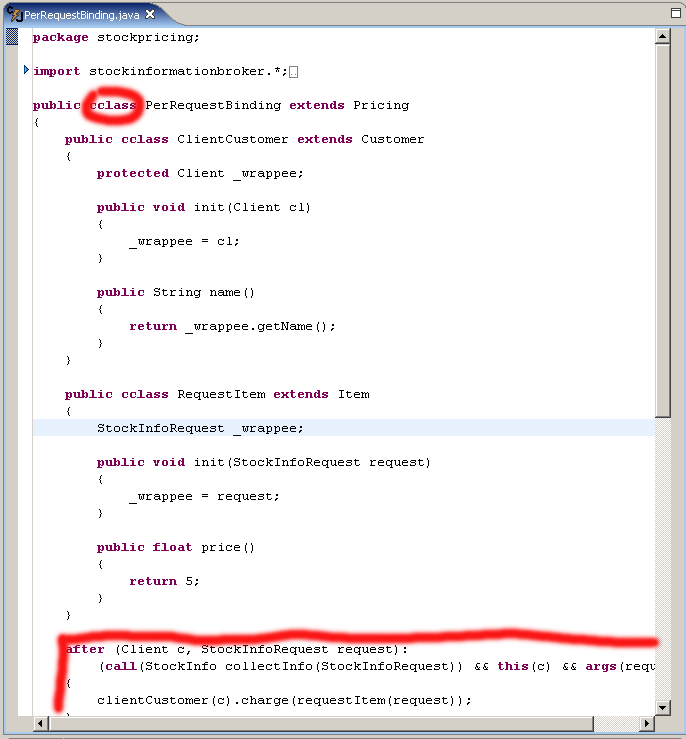
\includegraphics[width=0.60\textwidth]{images/hilight.png}
	\caption{Codehighlighting in \cjdt}
	\label{fig:hilight}
\end{figure*}

  \item Outline view showing structural members and crosscutting relationships. Also from an advice declaration to the places it advises. (Figure \ref{fig:outline})

\begin{figure*}[htbp]
	\centering
		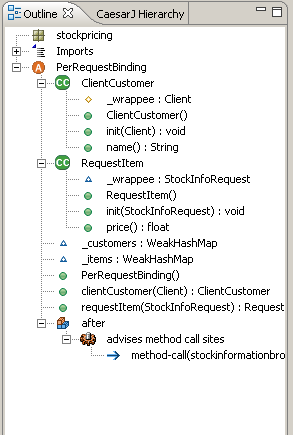
\includegraphics[width=0.35\textwidth]{images/outline.png}
	\caption{Outline view with advice relations}
	\label{fig:outline}
\end{figure*}

  \item New \caesarj -project wizard. This wizard helps you to start a new \caesarj -project. (Figure \ref{fig:projectwizard})
  
\begin{figure*}[htbp]
	\centering
		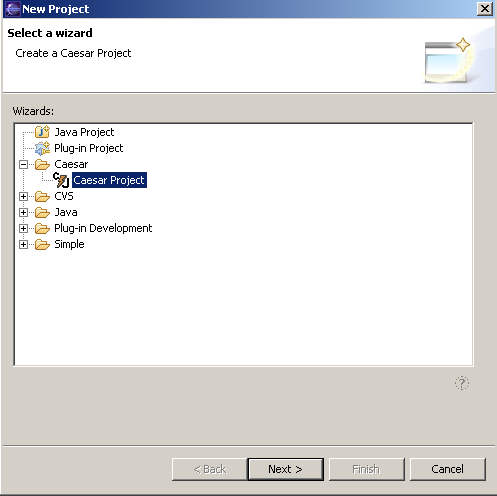
\includegraphics[width=0.60\textwidth]{images/project_wizard.png}
	\caption{New \caesarj -project wizard}
	\label{fig:projectwizard}
\end{figure*} 
     
  \item \caesarj ~hierarchy view. This view shows the multiple inheritance and nested class relations of an \caesarj ~top level class. (Figure \ref{fig:hierarchy})
  
\begin{figure*}[htbp]
	\centering
		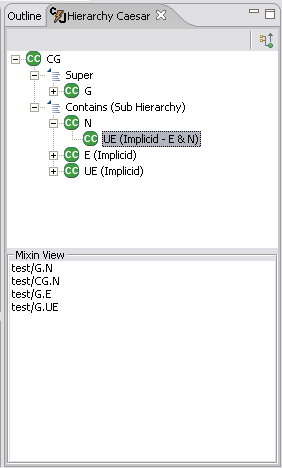
\includegraphics[width=0.35\textwidth]{images/hierarchy.png}
	\caption{\caesarj ~hierarchy view}
	\label{fig:hierarchy}
\end{figure*} 

  \item Debugging support. (Figure \ref{fig:debug1})
  
\begin{figure*}[htbp]
	\centering
		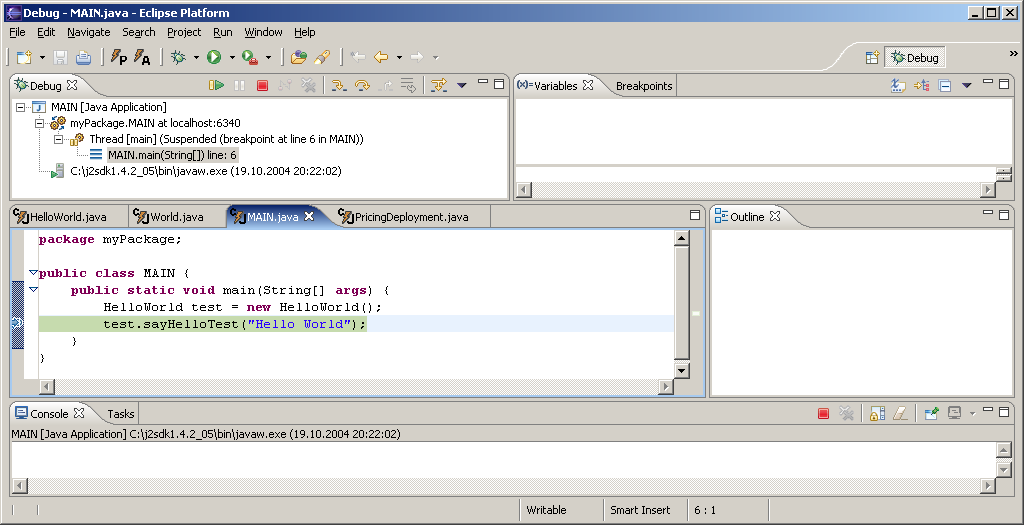
\includegraphics[width=1.0\textwidth]{images/debug1.png}
	\caption{Debugging an \caesarj -project}
	\label{fig:debug1}
\end{figure*}
\end{itemize}

\newpage
\section{\cjdt ~Installation}
The following two sections describe the installation of the \caesarj ~eclipse plugin. Two scenarios are possible: clean installation and updating an existing installation.
\subsection{Clean Installation} 
\cjdt is installed using the Eclipse Update Manager. We recommend you to use Eclipse 3.X.
\subsubsection{Using A Proxy Server} 
If you need to use a proxy server to access the internet, the first thing
to do is configure the proxy details so that the update manager can contact the
\cjdt ~update site. From the Window menu select preferences, and then the
Install/Update tab. Please enter your proxy server details as shown in fig \ref{fig:proxy}.
\begin{figure*}[htbp]
	\centering
		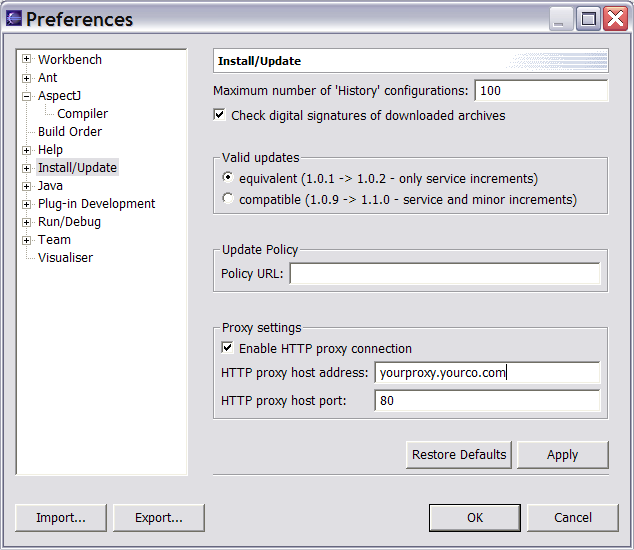
\includegraphics[width=0.80\textwidth]{./images/proxy.png}
	\caption{Setting up your proxy server}
	\label{fig:proxy}
\end{figure*}

\subsubsection{Install via Update Manager} 
Create an update site bookmark for the \cjdt ~update site, and start the install procedure.
% Ob man das brauch? \label{sec:In Eclipse 3.0}
From the help menu, select \markedtext{Software Updates} $\rightarrow$ \markedtext{Find and Install}. Select \markedtext{Search for new features to install} and click \markedtext{Next}.
Click \markedtext{Add Update Site} and enter the name \markedtext{\caesarj ~update site} and the folowing URL:  
\begin{center}
\href{http://cage.st.informatik.tu-darmstadt.de/caesar/updatesite/0.3.1}{http://cage.st.informatik.tu-darmstadt.de/caesar/updatesite/0.3.1}
\end{center}
Click \markedtext{OK}.
Fully expand the appearing \cjdt ~update site node and select \markedtext{\caesarj}. Click
\markedtext{Next}. Select \markedtext{org.caesarj.feature} as shown in figure \ref{fig:installpage30} and click \markedtext{Next}.\\

\begin{figure*}[htbp]
	\centering
		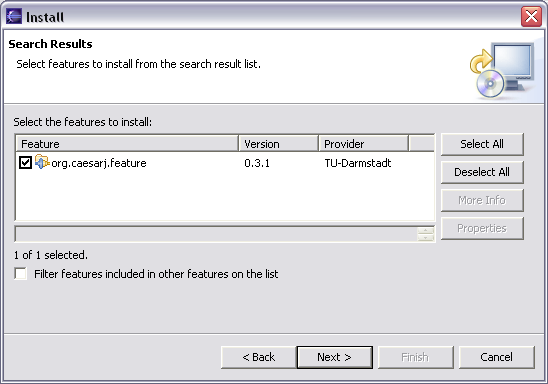
\includegraphics[width=0.85\textwidth]{./images/install_page_3_0.png}
	\caption{Selection of the \caesarj -plugin}
	\label{fig:installpage30}
\end{figure*}

Accept the \markedtext{license agreement} and proceed to the installation.

\subsection{Updating an Existing Installation}
Proceed as for a clean install, except that the \cjdt ~update site bookmark should already
exist. All you need to do, is to expand bookmark and go on. If the version you have
installed is the same as the version on the update site (or more recent even),
then you will not be presented with any install options.

\subsection{Is Everything OK?} 
Restart the Eclipse workbench. Try to open a new perspective by clicking \markedtext{Window} $\rightarrow$ \markedtext{Open Perspective}. Pick \markedtext{other} and select \markedtext{CaesarJ Perspective} in the upcoming list.
When the perspective opens successfully, the installation of your \cjdt ~works fine.
%\begin{figure}[htbp]
%	\centering
%		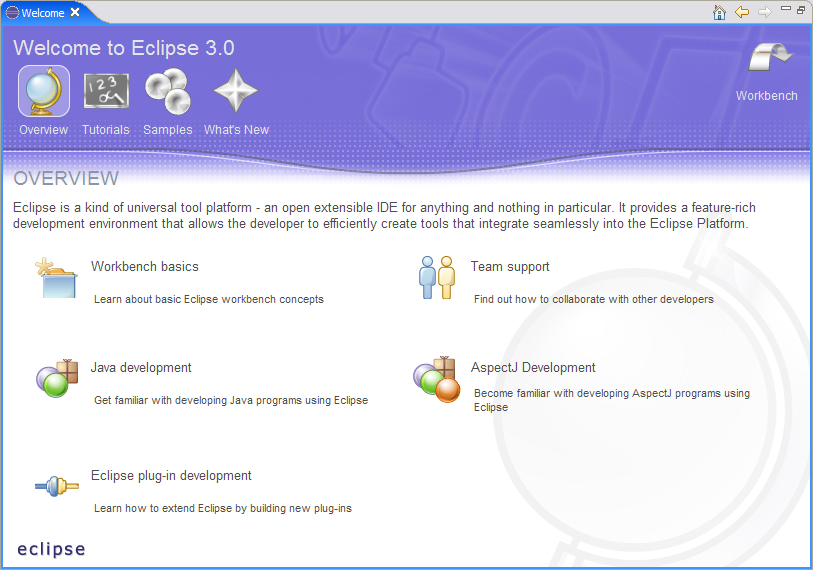
\includegraphics[width=0.95\textwidth]{./images/welcome_3_0.png}
%	\label{fig:welcome_3_0}
%\end{figure}



\newpage
\section{Features\label{features}}
The following section describes the extending features of the \cjdt ~Plugin.

\subsection{Opening the \caesarj -perspective}
First of all you need to open the \caesarj -perspective. It includes some new features like the \caesar -editor, the new outline view or the \caesarj -hierarchy view.\\
You can open this perspective by selecting: \markedtext{Window} $\rightarrow$ \markedtext{Open Perspective} $\rightarrow$ \markedtext{other} $\rightarrow$ \markedtext{CaesarJ perspective}.\\
If this is the first time you used the plugin, you will see the following dialog popup shown in figure \ref{fig:view_properties}.

\begin{figure}[htbp]
	\centering
		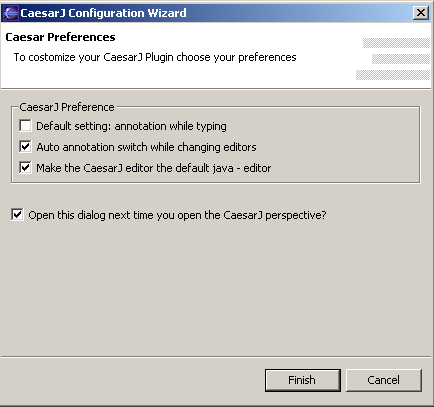
\includegraphics[width=0.5\textwidth]{images/view_properties.png}
	\caption{The \caesarj ~Preferences}	
	\label{fig:view_properties}
\end{figure}

This dialog configures some Eclipse settings that will make your life much easier when
working with CaesarJ projects. Leave everything selected and click
\markedtext{Finish}.

\subsection{Creating a new \caesarj project}
From the File menu select \markedtext{New} $\rightarrow$ \markedtext{Project}. Pick \markedtext{Caesar Project} in the list and select \markedtext{Next} as shown in figure \ref{fig:project_wizard}.

\begin{figure}[htbp]
	\centering
		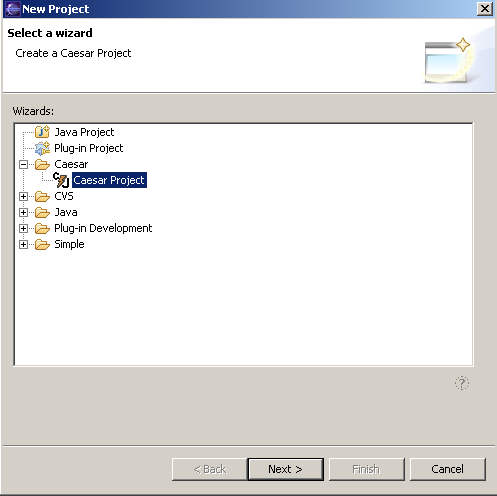
\includegraphics[width=0.70\textwidth]{images/project_wizard.png}
	\caption{Coosing the New Project Wizard}
	\label{fig:project_wizard}
\end{figure}

If it doesn't appear in the list, this is probably the first time you use the plugin. Select \markedtext{Other} and then \markedtext{Caesar} and \markedtext{Caesar Project}.\\
The wizard is opend. Here choose a name for your project as shown in figure \ref{fig:project_wizard2}.

\begin{figure}[htbp]
	\centering
		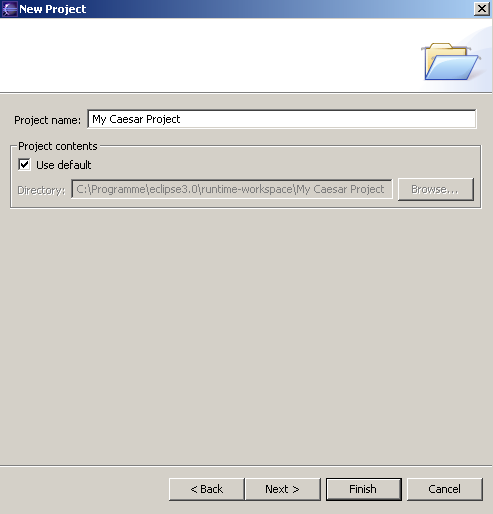
\includegraphics[width=0.70\textwidth]{images/project_wizard2.png}
	\caption{The New Project Wizard}
	\label{fig:project_wizard2}
\end{figure}

This wizard has identical behaviour to the new Java project wizard (except of course that
it creates a project with the Caesar nature).\\
When you click \markedtext{Finish}, your project will be created.


First, creat a package for your class.  Select the project you created in the package explorer, right click, and select
"New" -$>$ "Package" -$>$ "Other" from the context menu. You have to look for "Package" in the "Java" folder.\\\\
\begin{figure}[htbp]
	\centering
		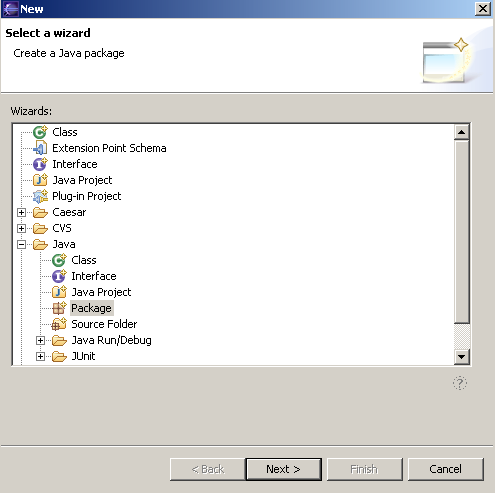
\includegraphics[width=0.70\textwidth]{images/package.png}
	\label{fig:package}
\end{figure}\\\\
Name the package "myPackage" then click finish.\\\\
Select the package you just created, and from the context menu select "New" -$>$ "Class". Name the
class "HelloWorld" and select the option to let Eclipse create a new main method for you. Click "Finish".\newpage
Edit the text in the editor so that it looks something like this:\\\\
\begin{center}
	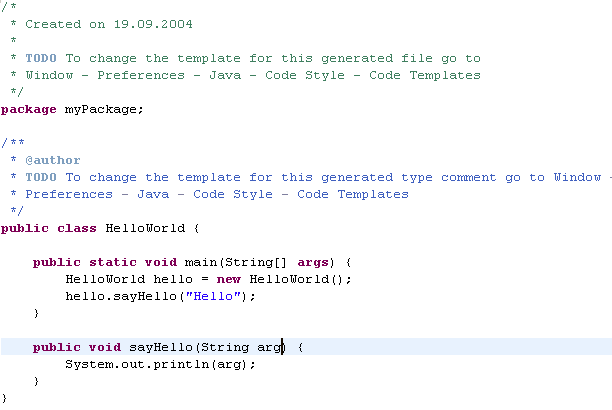
\includegraphics[width=0.80\textwidth]{images/code.png}
\end{center}
	
Save the file.\\\\

Notice that unlike in a Java project, there was no eager parsing of the buffer as you typed (the outline view didn't update). Your Eclipse workbench should be looking something like this:\\
\begin{center}
	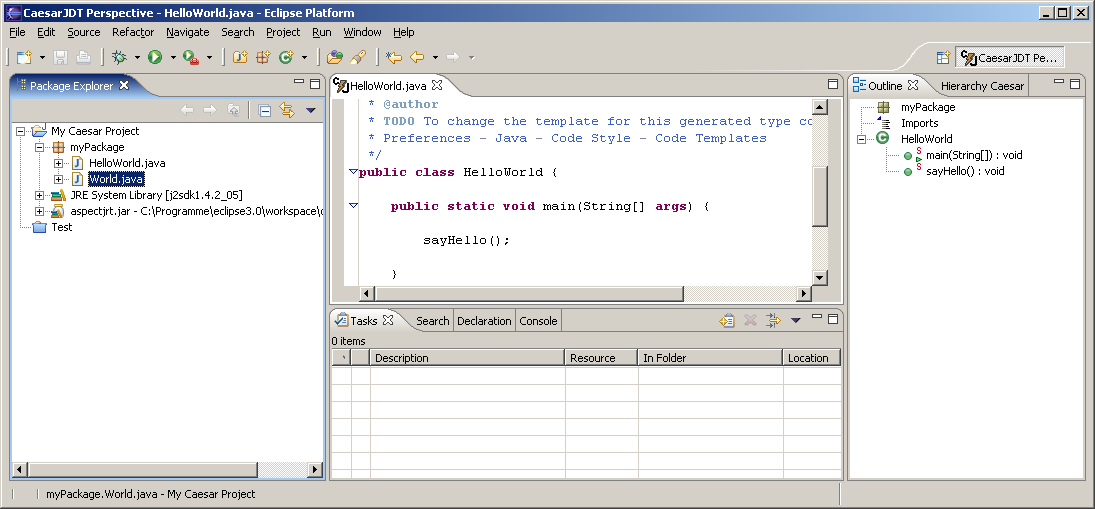
\includegraphics[width=1.0\textwidth]{images/workspace_newclass.png}
\end{center}

\subsection{Adding a New Aspect to Your Project}
Create a new Class and name it \code{World}. Edit the buffer so it looks as follows and then save it:\\\\
\begin{lstlisting}[basicstyle=\small\it,caption=Parser endElement Event,label=lst:endelement,name=listing:endelement,frame=none]{}
package myPackage;
//TEST
public cclass World { 	
      after(HelloWorld c, String a) :
      	(call(void sayHello(String)) && this(c) && args(a))
		{
            System.out.println("Hello to you too...");
		}
}\end{lstlisting}
%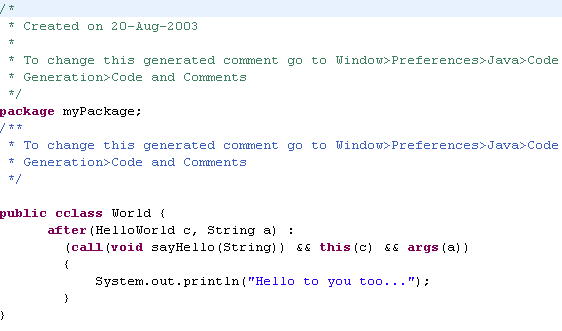
\includegraphics[width=0.80\textwidth]{images/aspect.png}\\

Make a clean Build of the project, and the outline view populates. Expand the \code{after()} node.\\\\
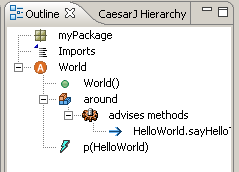
\includegraphics[width=0.5\textwidth]{images/aspect2.png}\newpage

You can see that this advice is affecting the HelloWorld.sayHello() method. Clicking on the \code{HelloWorld.sayHello()} node in the outline takes you to the declaration of HelloWorld.sayHello().

Notice the \code{advice annotation} in the editor buffer (highlighted) and that the \code{sayHello} method in the outline view shows that it is advised by the World aspect.\\\\
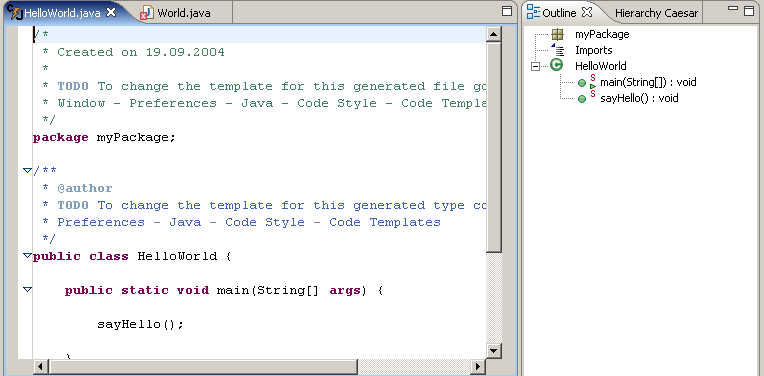
\includegraphics[width=0.95\textwidth]{images/aspect3.png}\\\\

Selecting the \code{World.after()} node in the outline view takes you back to the advice declaration. Right-clicking on the advice annotation brings up a context menu that also allows you to navigate to the advice.\\\\
\textbf{TODO BILD FEHLT KONNTE ICH NICHT SCREENSHOOT MACHEN  Weil es nicht geht EDITOR mit ADVICE CONTEXT}



\subsection{Running an \caesarj ~Program}
Select your \caesarj ~project in the Package Explorer. Drop-down the \markedtext{Run} icon on the toolbar and click \markedtext{Run...}\\
Select \markedtext{Java Application} in the left-hand tab and click \markedtext{New}.
Name this configuration \code{HelloWorld} and then click \markedtext{Search} to find the main class. Select \code{HelloWorld} as described in figure \ref{fig:run}.

\begin{figure*}[htbp]
	\centering
		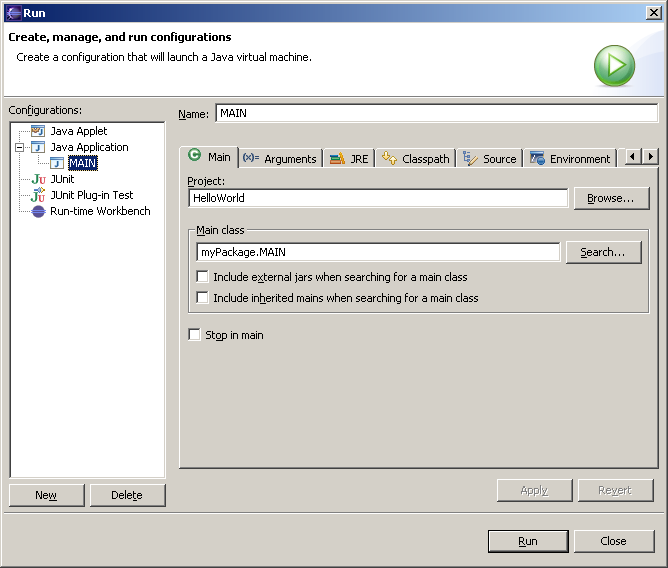
\includegraphics[width=0.60\textwidth]{images/run.png}
	\caption{Running a \caesarj ~program}
	\label{fig:run}
\end{figure*}

Click \markedtext{Apply} and then \markedtext{Run}.\\
You should see the output of the \code{HelloWorld} ~class and the \code{World} ~aspect in the console like shown in figure \ref{fig:console}.

\begin{figure*}[htbp]
	\centering
		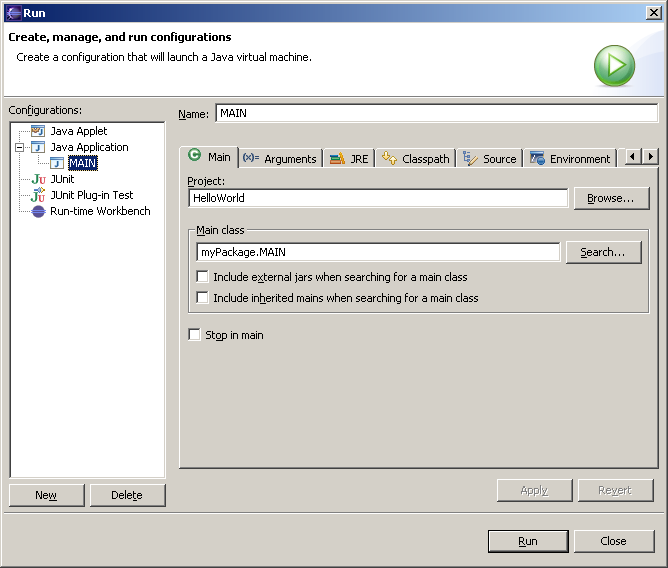
\includegraphics[width=0.60\textwidth]{images/run.png}
	\caption{Programs output}
	\label{fig:console}
\end{figure*}
To run this configuration again, just click on the \markedtext{Run} icon placed on the toolbar.


\subsection{Debugging Caesar Programs}
You can debug Caesar programs using the normal Java debugger. To set a breakpoint, right-click in the gutter of the editor and choose \markedtext{Toggle Breakpoint}(see figure \ref{fig:brake_point}). Another possibility is a simply double-click on the gutter.
\begin{figure*}[htbp]
	\centering
		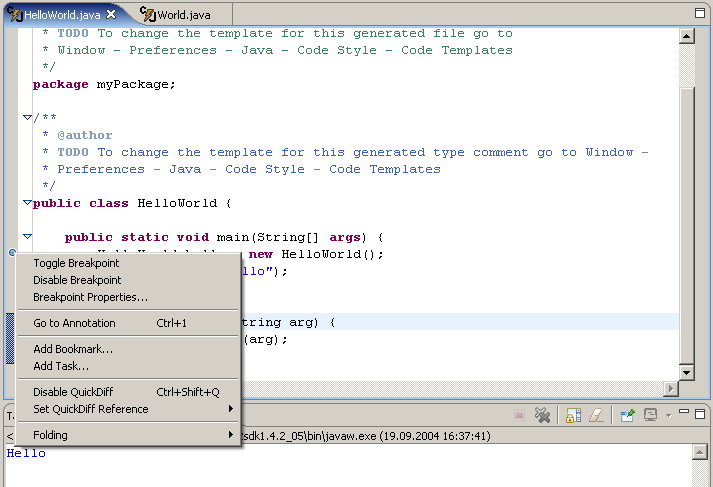
\includegraphics[width=0.80\textwidth]{images/brake_point.png}
	\caption{Toggling a debugging breakpoint}
	\label{fig:brake_point}
\end{figure*}

With one or more breakpoints set, you launch the Eclipse debugger in the normal way by clicking on the debug icon in the toolbar. The debugger perspective looks like figure \ref{fig:debuger}.
\begin{figure*}[htbp]
	\centering
		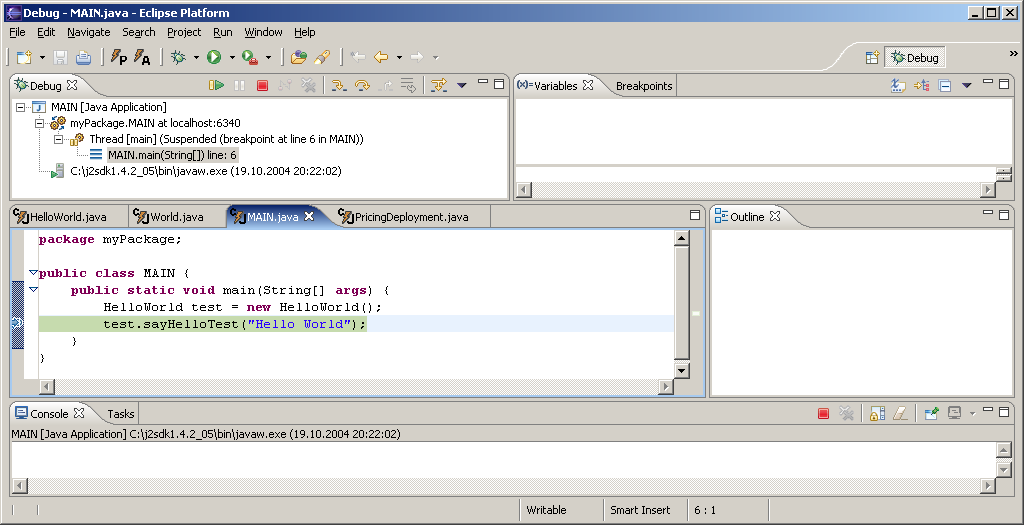
\includegraphics[width=0.80\textwidth]{images/debug1.png}
	\caption{Debugger perspective}
	\label{fig:debuger}
\end{figure*}

You can use the Java Debug step filters (\markedtext{Window} $\rightarrow$ \markedtext{Preferences} $\rightarrow$ \markedtext{Java} $\rightarrow$ \markedtext{Debug} $\rightarrow$ \markedtext{Step Filtering}) to make this process a little easier.\\
Note: A current limitation is that you cannot step into advices.

\newpage
\section{Properties and Shortcuts}
If you have opened the Caesar Perspective, there are some configurations left. Open \markedtext{Window} $\rightarrow$ \markedtext{Customise Perspective}. Check the \markedtext{Caesar} check box as shown in figure \ref{fig:propert}.

\begin{figure*}[htbp]
	\centering
		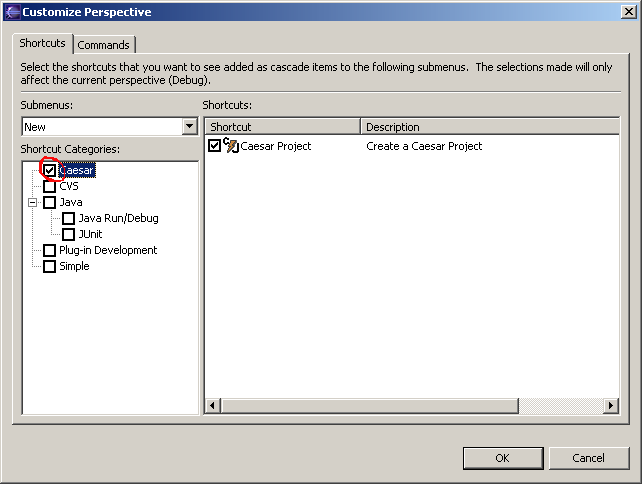
\includegraphics[width=0.60\textwidth]{images/propert.png}
	\caption{Selection the \caesarj ~perspective}
	\label{fig:propert}
\end{figure*}

If this is done, two new Buttons will appear in the tool bar like in figure \ref{fig:toolbar}.

\begin{figure*}[htbp]
	\centering
		
\includegraphics[width=1.0\textwidth]{images/toolbar.png}
	\caption{\caesarj ~tool bar shortcuts}
	\label{fig:toolbar}
\end{figure*}

Figure \ref{fig:properties} shows the \caesarj -Configuration-Wizard, which will be displayed by pressing the \markedtext{P}-Button.

\begin{figure*}[htbp]
	\centering
		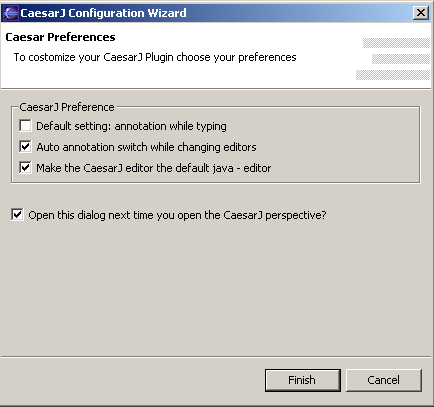
\includegraphics[width=0.60\textwidth]{images/view_properties.png}
	\caption{\caesarj -Configuration-Wizard}
	\label{fig:properties}
\end{figure*}

The \markedtext{A}-Button toggles the "Annotation-While-Typing" option on or off. Even for the Java-Editor.\\
A main feature of the \cjdt ~is the automatic annotation toggling while switching between the \caesarj - and the JAVA-editor. This is a useful feature, because the \cjdt does not support live annotation yet. In this way, \caesarj ~syntax are not marked as wrong expressions.




\newpage
\section{Using the Visualiser and views}
If this is the first time you use the \cjdt, switch to the \caesarj ~perspective by selecting \markedtext{Window} $\rightarrow$ \markedtext{Open Perspective} $\rightarrow$ \markedtext{Other}. Pick \markedtext{CaesarJDT Perspective} (see figure \ref{fig:select_persp}) in the list.

\begin{figure*}[htbp]
	\centering
		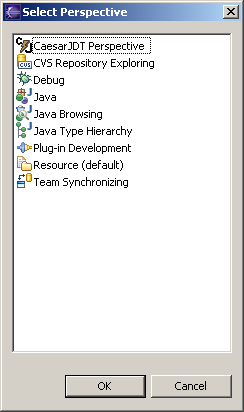
\includegraphics[width=0.35\textwidth]{images/select_persp.png}
	\caption{Perspective selection}
	\label{fig:select_persp}
\end{figure*}

This perspective extends the Java perspective. Especially a new view is available. The \markedtext{\caesarj ~Hierarchy View}. See section \ref{hierarchyview} for detailed information.\\
You can switch between the Java and Caesar Visualization perspectives using the perspective icons in the top right of the menu bar.\\
\subsection{Outline view}
The outline view is showing structural members and crosscutting relationships. It extends the Java outline view by additional information (e.g advice declarations to the places it advises). A sample outline view bar is shown in figure \ref{fig:outline_view}. \textbf{TODO Bild noch nicht das richtige.}\\

\begin{figure*}[htbp]
	\centering
		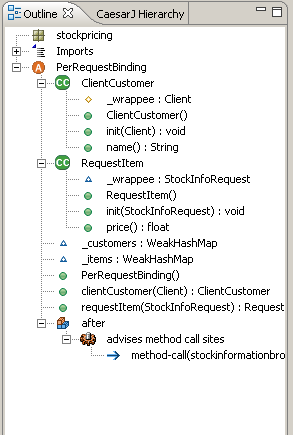
\includegraphics[width=0.35\textwidth]{images/outline.png}
	\caption{Outline View}
	\label{fig:outline_view}
\end{figure*}

\subsection{Hierarchy View\label{hierarchyview}}
% It displays the hierarchical relationships of \caesarj ~cclasses.
A \caesarj ~hierarchy view displays the hierarchical relationships of \caesarj ~cclasses. That means, that for each cclass their super-classes are displayed under the \markedtext{Super} node (see figure \ref{fig:hierarchy_view}). If the class contains nested classes (\markedtext{Contains} node) there are two displaying modes available for them:
\begin{itemize}
	\item[\textbf{Super:}] For each nested class their super classes are displayed.
	\item[\textbf{Sub:}] For each nested class their sub classes are displayed. If a sub class has two super classes the linearized inheritance relation is displayed in brackets after the class name.
\end{itemize}

\begin{figure*}[htbp]
	\centering
		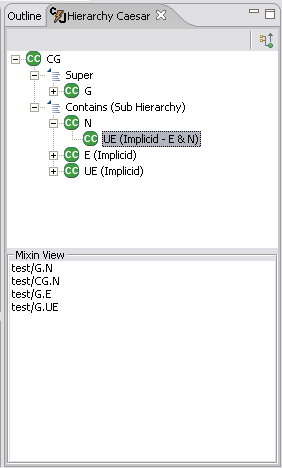
\includegraphics[width=0.35\textwidth]{images/hierarchy.png}
	\caption{\caesarj ~hierarchy view}
	\label{fig:hierarchy_view}
\end{figure*}

The modes can be switched by pressing the control button in the upper-right of the view. The second part of the view, named "Mixin view", shows the mixin composition of the currently selected (nested-) cclass.\\
\textbf{Note:} Because this view needs meta information from the compiler, the view refreshes when a project was (re-)built successfully.



\end{document}